%!TEX root = ../../proposal.tex
\clearpage
\section{Introduction}
\begin{body}
	Micro computed tomography ($\mu$CT) is a widely used modality in industry and research. For the latter, it enables the study of small structures in animals, for example rodents such as mice\cite{percianoInsight3DMicroCT2017}.
	A common task while performing short-term or long-term studies with mice is the segmentation of the image data, as it is an important step for quantitative image analysis\cite{sheppardTechniquesHelicalScanning2014}. Segmentation can be defined as the process of separating various image components and extracting parts that are of interest for later analysis\cite{percianoInsight3DMicroCT2017}.
	\newline
	There exist a few free and open-source programs capable of segmenting $\mu$CT datasets.
	The two actively maintained and well-known\cite{mandoliniComparisonThree3D2022,virziComprehensiveReview3D2020} software packages are:
	\begin{itemize}
		\item \textsc{ITK-SNAP}\cite{yushkevichUserguided3DActive2006} available under the \texttt{GNU General Public License}\cite{licenseGnuGeneralPublic1989}
		\item \textsc{3D Slicer}\cite{kikinis3DSlicerPlatform2014} available under a \texttt{BSD style license}\cite{gaudeulPublicProvisionPrivate2005}
	\end{itemize}
	Both provide the user with a plethora of segmentation algorithms which can be grouped into manual, semi-automatic and fully automatic. They provide several tools capable of complex segmentation workflows\cite{percianoInsight3DMicroCT2017}.
	Accuracy and efficiency of the segmentation however strongly depend on user experience and the segmentation algorithm chosen\cite{mandoliniComparisonThree3D2022,aydinRELIABILITYREPRODUCIBILITYTIMEEFFICIENCY2020}. Despite this fact, there is a distinct lack of general recommendations, instructions or guides on how to efficiently segment $\mu$CT datasets.\\
	For example, searching for:
	\begin{displayquote}
	  micro ct 'segmentation instructions'
    \end{displayquote}
	or
    \begin{displayquote}
	  micro ct 'segmentation guide'
    \end{displayquote}
	on Google Scholar returns a total of 6 and 27 search results respectively.
	3D Slicers documentation website\cite{pinterPolymorphSegmentationRepresentation2019} explains the software and many of the available tools in the standard distribution of 3D Slicer. But it does not feature a recommended segmentation workflow.
  \end{body}
\section{Problem Statement}
\begin{body}
	As mentioned above, \texttt{3D Slicer} and \texttt{ITK-SNAP} provide the user with a sizable amount of segmentation tools and the selection of the correct segmentation algorithm and workflow have a non-negligible influence on the segmentation quality as well as the time the user has to spend on it.
	Therefore, we hypothesize that users of \texttt{3D Slicer} will benefit from a streamlined segmentation guide, and it will improve segmentation quality as well as workflow efficiency.
\end{body}
\clearpage
\section{Objectives and Aims}
\begin{body}
  The master thesis is based on the following hypothesis:
  \begin{itemize}
	\item A segmentation guide will improve segmentation accuracy for inexperienced users
  \end{itemize}
  Similar to Guindon et al.\cite{diceMeasuresAmountEcologic1945}, we plan to evaluate segmentation accuracy by comparing the results of the test candidates with the author's ground truth segmentation. Evaluation will be done by calculating the Dice coefficient\cite{diceMeasuresAmountEcologic1945} or Hausdorff distance\cite{birsanOneHundredYears2006} of the two segmentation results and correlating the error with literature\cite{kenneyHighthroughputSemiautomatedBone2022}. The resulting ground truth segmentations can then be used in later works. For instance as a training dataset for an deep-learning based approach as Rushmore et al. point out\cite{rushmoreAnatomicallyCuratedSegmentation2022}.
\end{body}
\clearpage
\section{Literature to be reviewed}
\begin{body}
	The sources of literature used for this master thesis are PubMed, ScienceDirect, IEEE Xplore and the meta-search engine Google Scholar.
	The main workflow of searching for appropriate literature was to search for publications covering the defined keywords\ref{s:Keywords} in the abstract, reading as many of the papers as possible and filtering out the most relevant.
	The following papers are the result of this workflow at the current time:
	\begin{itemize}
		\item Comparison of segmentation tools for structural analysis of bone tissues by finite elements (Argüello et al. \textsf{\textbf{Journal of Physics}})
		\item Comprehensive Review of 3D Segmentation Software Tools for MRI Usable for Pelvic Surgery Planning (Virzì et al. \textsf{\textbf{Journal of Digital Imaging}})
		\item Comparison of Three 3D Segmentation Software Tools for Hip Surgical Planning (Mandolini et al. \textsf{\bfseries{MDPI}})
		\item Morphological mouse phenotyping: anatomy, histology and imaging (Ruberte et al. \textsf{\bfseries{Academic Press}})
		\item User-guided 3D active contour segmentation of anatomical structures: Significantly improved efficiency and reliability (Yushkevich et al. \textsf{\bfseries{NeuroImage}})
		\item Medical image segmentation on GPUs – A comprehensive review (Smistad et al. \textsf{\bfseries{Medical Image Analysis}})
		\item Segmentation and Visual Analysis of Whole-Body Mouse Skeleton microSPECT (Khmelinskii et al. \textsf{\bfseries{PLoS ONE}})
		\item SlicerRT: Radiation therapy research toolkit for 3D Slicer (Pinter et al. \textsf{\bfseries{Medical Physics}})
		\item Insight into 3D micro-CT data: exploring segmentation algorithms through performance metrics (Perciano et al. \textsf{\bfseries{Journal of Synchrotron Radiation}})
		\item SAMM (Segment Any Medical Model): A 3D Slicer Integration to SAM (Liu et al. \textsf{\bfseries{Johns Hopkins University}})
	\end{itemize}
\end{body}

\clearpage
\section{Research design and Methods}
\begin{body}
	The practical work for this project will be completed by the author on his private computer.
	The first step will be the segmentation of the $\mu$CT scans, which will serve as a ground truth and finding possible efficient workflows with the tools included in \texttt{3D Slicer}.
	Then a guide will be created outlining 2-3 different possible workflows for bone segmentation.
	This guide will be handed out to test candidates in conjunction with the task of using the guide to segment a specific part of a scan volume.
	The candidates are asked to perform the segmentation and return their results to the author, who will then calculate their accuracy by comparing the result of each test candidate with his own segmentation. Testers will also be asked to take note of the time it took them to complete the segmentation task. A qualitative score of the segmentation will be created by computing a score like the Hausdorff distance\cite{birsanOneHundredYears2006} or the Dice coefficient\cite{diceMeasuresAmountEcologic1945}. Either of the scores will be computed using the \texttt{SlicerRT}\cite{pinterSlicerRTRadiationTherapy2012} Extension for the 3D Slicer software package.
\end{body}

\section{Outcome}
\begin{body}
	As creating as general segmentation guide for $\mu$CT scans of mice and educating the user on every possible segmentation method for every tissue is far beyond the capabilities of this master thesis, the outcome should be twofold:
	\begin{enumerate}
		\item Educating users of segmentation software like 3D Slicer on the capabilities and correct usage of their tools
		\item Enabling further research on the topic of $\mu$CT segmentation for different tissues and segmentation methods and algorithms
	\end{enumerate}
\end{body}

\clearpage
\section{Study Period}
\subsection{Milestones}
\begin{body}
	\begin{itemize}
		\item Find supervisor and topic in September 2023
		\item Submission of the abstract in November 2023
		\item Submission of the research proposal in February 2024
		\item Finishing Segmentation work in April 2024
		\item Finishing Guide evaluation at the end of May 2024
		\item Finish the first version of the thesis in June 2024
		\item Submission of the final thesis in July 2024
	\end{itemize}
\end{body}

\subsection{Chart}
\begin{body}
	The segmentation work and literature search is planned to be finished by the end of April 2024.
	After the segmentation work is done the guide will be tested and evaluated from April 2024 until June 2024.
	Writing of the thesis starts with February 2024 and should be finished by June or July 2024.
	The final examination should at the latest take place in October 2024.
	\newline
	\newline
	\noindent
	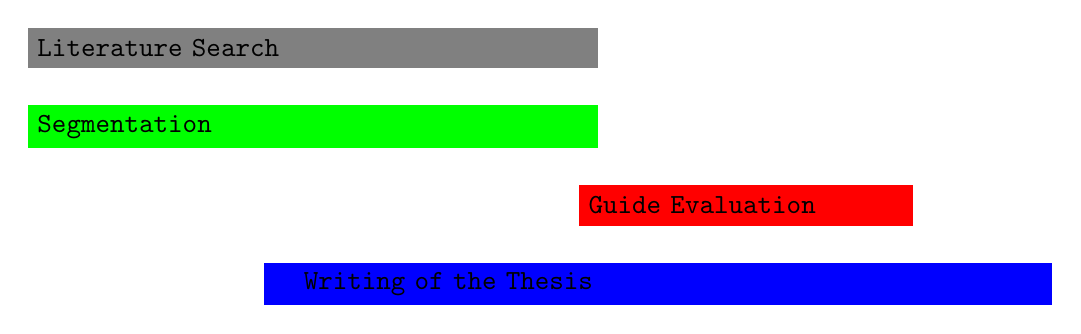
\begin{tikzpicture}
		\node at (0,0) [right=3cm,rectangle,draw=blue,fill=blue,minimum width=10cm,minimum height=0.5cm,text width=9cm] {\texttt{Writing of the Thesis}};
		\node at (0,3) [right=0cm,rectangle,draw=gray,fill=gray,minimum width=7cm,minimum height=0.5cm,text width=7cm] {\texttt{Literature Search}};
		\node at (0,2) [right=0cm,rectangle,draw=green,fill=green,minimum width=7cm,minimum height=0.5cm,text width=7cm] {\texttt{Segmentation}};
		\node at (0,1) [right=7cm,rectangle,draw=red,fill=red,minimum width=4cm,minimum height=0.5cm,text width=4cm] {\texttt{Guide Evaluation}};
	\end{tikzpicture}
	\newline
	\noindent
	\begin{tikzpicture}
		\draw [line width=0.5mm] (0,0) -- (15,0);
		\foreach \x in {1,3,5,7,9,11,13}
		\draw [line width=0.5mm](\x cm,5pt) -- (\x cm,-5pt);
		\draw (1,0) node[below=3pt] {$\begin{turn}{45}January 2024\end{turn}$};
		\draw (3,0) node[below=3pt] {$\begin{turn}{45}February 2024\end{turn}$};
		\draw (5,0) node[below=3pt] {$\begin{turn}{45}March 2024\end{turn}$};
		\draw (7,0) node[below=3pt] {$\begin{turn}{45}April 2024\end{turn}$};
		\draw (9,0) node[below=3pt] {$\begin{turn}{45}May 2024\end{turn}$};
		\draw (11,0) node[below=3pt] {$\begin{turn}{45}June 2024\end{turn}$};
		\draw (13,0) node[below=3pt] {$\begin{turn}{45}July 2024\end{turn}$};
	\end{tikzpicture}
\end{body}
